% Define document class. Important.
\documentclass[a4paper,twoside,openright]{report}

\usepackage{acronym}

% Margener
%\setlength{\evensidemargin}{1cm}
%\setlength{\oddsidemargin}{1cm}

% Set up encoding. Latin1 since UTF-8 is fuckably difficult to work with.
\usepackage[utf8x]{inputenc}
%\usepackage[T1]{fontenc}
% Load up bibliography.
\usepackage[authoryear]{natbib}
\setcitestyle{numbers,square}
% Bibliography style.
\bibliographystyle{plainnat}

% Algorithm support.
\usepackage{algorithmic}
\usepackage{algorithm2e}
\usepackage{subfig}
\usepackage{amsmath}
\usepackage{amsfonts}


% Image frames.
\setlength{\fboxsep}{0pt}
\setlength{\fboxrule}{0.5pt}

% Also, images.
\usepackage{graphicx}

% tabeller der strækker sig over flere sider
\usepackage{longtable}

% flere tabel-muligheder
\usepackage{multirow}

% bedre enumerate
\usepackage{enumitem}

% Todo notes here and there.
% write instead for disable: \usepackage[disable]{todonotes}
\usepackage[disable]{todonotes}

% Forbedrede floats.
\usepackage{float}
\usepackage{rotating}

% Special symbols availability.
\usepackage{amssymb}

\usepackage{textcomp}

% CODE %
\usepackage{listings}
\usepackage[scaled]{beramono} % Better font for listings
\usepackage{color}
\definecolor{gray}{rgb}{0.4,0.4,0.4}
\definecolor{darkblue}{rgb}{0.0,0.0,0.6}
\definecolor{cyan}{rgb}{0.0,0.6,0.6}
\lstset{
  tabsize=4,
  breaklines=true,
  numbers=left,
  captionpos=b,
  stepnumber=1,
  numbersep=10pt,
  showstringspaces=false,
  basicstyle=\footnotesize,
}% Neat-o referencer...o.
\usepackage{bookmark,hyperref}
\usepackage{nameref}

% hack fra nettet.
% http://tex.stackexchange.com/questions/1230/reference-name-of-description-list-item-in-latex
\makeatletter
\let\orgdescriptionlabel\descriptionlabel
\renewcommand*{\descriptionlabel}[1]{
  \let\orglabel\label
  \let\label\@gobble
  \phantomsection
  \edef\@currentlabel{#1}
  %\edef\@currentlabelname{#1}
%  \let\label\orglabel
  \orgdescriptionlabel{#1}
}
\makeatother
% Rettehak. Meget lettere end \checkmark
\newcommand{\yes}{\checkmark}

\pagenumbering{arabic} % Ensure page numbering in our desired form.

% New command for two figures, side by side.
\newcommand{\twofigs}[6]
{
	\begin{figure}[H]
		\begin{minipage}[b]{0.5\columnwidth}
		\centering\fbox{\includegraphics[width=0.8\columnwidth]{img/#1}}\caption{#2\label{#3}}
		\end{minipage}
		\hspace{0.5cm}
		\begin{minipage}[b]{0.5\columnwidth}
		\centering\fbox{\includegraphics[width=0.8\columnwidth]{img/#4}}\caption{#5\label{#6}}
		\end{minipage}	\end{figure}
}

% Sørg for at paragrafplads ikke spildes.
\raggedbottom
\usepackage[titletoc]{appendix}

% Package til at regne forskellen ud mellem 2 labels
\usepackage{refcount}
\newcommand{\pagedifference}[2]{\number\numexpr\getpagerefnumber{#2}-\getpagerefnumber{#1}\relax}

% Opsætning af autoref%
\def\figureautorefname{Figure}
\def\tableautorefname{Table}
\def\chapterautorefname{Chapter}
\def\sectionautorefname{Section}
\def\subsectionautorefname{Subsection}

%Ingen indentering
\setlength{\parindent}{0mm}


\begin{document}
\acrodef{crud}[CRUD]{Create, Read, Update, Delete}
\acrodef{api}[API]{Application Programming Interface}
\acrodef{json}[JSON]{JavaScript Object Notation}
\acrodef{xml}[XML]{Extensible Markup Language}
\acrodef{api}[API]{Application Programming Interface}
\acrodef{cat}[CAT]{Category Administration Tool}
\acrodef{lamp}[LAMP]{Linux, Apache2, MySql and PHP}
\acrodef{giraf}[GIRAF]{Graphical Interface Resources for Autistic Folk}
\acrodef{oha}[OHA]{Open Handset Alliance}
\acrodef{gui}[GUI]{Graphical User Interface}
\acrodef{json}[JSON]{JavaScript Object Notation}
\acrodef{foss}[FOSS]{Free and Open-Source Software}
\acrodef{ui}[UI]{User Interface}

\pagestyle{empty}

\thispagestyle{empty}
\begin{flushright}
\vspace{3cm}

\phantom{hul}

\phantom{hul}

\phantom{hul}

\textsl{\Huge WASTELAND}\\ \vspace{0.3cm}
\textsl{\Huge - A GIRAF Database} \vspace{0.5cm}

\rule{13cm}{3mm} \\ \vspace{1.5cm}
\vspace{1cm}

%Insert image here!
%\includegraphics[width=1.0\textwidth]{img/image} 

\vspace{1.5cm} 
\textsc{\Large P6 Project \\
Group SW603 \\
Department of Computer Science\\
Aalborg University\\
Some date 2013\\}
\end{flushright}

\cleardoublepage

% Dette er LaTeX-versionen af titelbladet for tek-nat-basis-rapporter 2004 efterår
% Filen kræver:
% Universitetets logo:  aau-logo.png (for LaTeX) eller aau-logo.ps (for LaTeX)
% Synopsis: En fil ved navn synopsis.tex

% Udarbejdet af: Hans Hüttel (hans@cs.auc.dk) 21. maj 2003
% Rettet af Morten Christophersen (mortench@tnb.aau.dk) 30. nov 2004(Ændret til nyt design 2004 efterår)

\phantomsection
\pdfbookmark[0]{Titlepage}{titlepage}
\thispagestyle{empty}
%\begin{titlepage}
\begin{nopagebreak}
{\samepage 
\begin{tabular}{r}
\parbox{\textwidth}{  \raisebox{11mm}{
\includegraphics[height=1.2cm]{img/aau-logo-1.png}}\\
\hfill \parbox{8cm}{\begin{tabular}{l} %4.90
{\small \textbf{Institut for Computer Science}}\\
{\small Selma Lagerlöfs Vej 300} \\
{\small 9220 Aalborg Ø} \\
{\small Phone 99 40 99 40} \\
{\small Fax 99 40 97 98} \\
{\small http://www.cs.aau.dk/}
\end{tabular}}}

\end{tabular}

\begin{tabular}{cc}
\parbox{7cm}{
\begin{description}

\item { Title:} 

WASTELAND - A GIRAF Database \\
  
\item { Theme:} 

Developing Complex Software Systems

\end{description}

\parbox{8cm}{

\begin{description}
\item { Project period:}\\
   6th semester 2013 SW
  \hspace{4cm}
\item { Project group:}\\
  SW603F13
  \hspace{4cm}
\item { Group members:}\\
Barbara Flindt\\
Hilmar Laksá Magnussen \\
Jeppe Blicher Tarp \\
Simon Jensen\\
  \hspace{2cm}
\item { Counselor:}\\
 Katja Hose\\
  
\end{description}
}
\begin{description}
\item { Circulation: 6 }
\item { Number of pages: 103 } 
\item { Number of Appendices: 3} 
\item { Finished } 4th of June 2013
\end{description}
\vfill } &
\parbox{7cm}{
  \vspace{.15cm}
  \hfill 
  \begin{tabular}{l}
  { Abstract:}\bigskip \\
  \fbox{
    \parbox{7cm}{\bigskip
     {\vfill{\small We describe the design and implmentation of a central server application for the GIRAF system with a database, an API for communication and synchronization between the central database and a local counterpart on an Android device. This is done in the context of a multiproject consisting of 8 groups, all working on various aspects of the GIRAF system. We end up with a working implementation and describe future work and tips for future students working on top of this project.
     \bigskip}}
     }}
   \end{tabular}}
\end{tabular}}
\\ \\ \\ \\ \\ \\ \\
\noindent{\footnotesize{\textit{Rapportens indhold er frit tilgængeligt, men offentliggørelse (med kildeangivelse) må kun ske efter aftale med forfatterne.}}}
\end{nopagebreak}
%\end{titlepage}

\cleardoublepage

\listoftodos
\chapter*{Preface}



\cleardoublepage
\pdfbookmark{Table of Contents}{toc}
\tableofcontents
\cleardoublepage
\pagestyle{plain}

%input main content here
\chapter{The GIRAF Project}\label{cha:common}

\ac{giraf} started out in 2011 as a semester project targeting children with autism and their guardians. %Allthough solutions exists these were expensive and did not provide the needed level of user-customization\todo{Er dette virkelig korrekt?}.
 In the following chapter, the overall vision for the \ac{giraf} project will be presented, the projects from previous years will be explained briefly along with the platform for the project. Lastly a section describing autism is included.


%% \todo{Write a little section about the contents of this chapter.}

%% \todo{Figure out which order this should be in}

\section{Vision for \acs{giraf}}
The vision for \ac{giraf} is to create a multi-purpose application based on \emph{Android} that can simplify and ease the lives of autistic children and their guardians.

The purpose of \ac{giraf} is to replace physical items that are being used daily by the children and their guardians with digitized versions. The idea being to gather several functionalities in one object and allowing customization for each individual child.

This will also optimize work procedures on the individual institution in such a way, that guardians will save time doing repetitive tasks such as making pictograms. This time could be spent with the children instead.

As of the spring of 2013 three schools and institutions for children with autism in Northern Jutland are involved in the development, but the hope is that \ac{giraf} will be distributed across all similar institutions in Denmark.


\section{Previous Years}
%This section briefly describes the projects developed for the \ac{giraf} project during 2011 and 2012.

During the first year of development, four parts of the \ac{giraf} project were developed. The four projects were developed during the spring semester of 2011 and included the projects:
\begin{description}
\item [Admin] An administration interface used for administrating different aspects of the \ac{giraf} system.
\item [DigiPECS] A digitized version of ``Picture Exchange Communication System''\cite{pecs} a system used as an aid for communication with people with special needs such as autism.
\item [Launcher] A home screen application and distribution platform for Android.
\item [aSchedule] A visual schedule for the Android platform.
\end{description}

During the spring semester of 2012, five new software groups continued development of the \ac{giraf} project. The projects developed during 2012 were:

\begin{description}
\item [Launcher] An enhancement of the launcher project developed during the spring semester of 2011.
\item [Oasis] An enhancement of the admin project from 2011. Furthermore the Oasis project developed a local database for the \ac{giraf} system.
\item [Parrot] An enhancement of the DigiPECS project from 2011. The project was renamed because of trademark issues.
\item [Savannah] A server side database with web interface for the \ac{giraf} system.
\item [Wombat] An Android application for measuring and visualizing time.
\end{description}

%During the spring semester of 2012, two different projects working with databases were developed although the databases from the two projects were never made able to synchronize.
During the spring semester of 2012 two databases were developed, however synchronization between them was never achieved.

\subsection*{Problems with Initial Implementation}
As the spring semester of 2013 started, an ''install party'' for the students was held. The party was intended to help the students compile and deploy the projects from 2012.

Even though a representatives for each of the 2012 groups were present, some compilation problems still occurred.

The repository used for distributing in 2012, was disorganized and difficult to navigate, i.e. due to:
\begin{itemize}
  \item Multiple copies of the same project.
  \item Unclear dependencies among the different project.
  \item Projects only meant to be compiled from Eclipse for Windows.
\end{itemize}

During the following week a working workspace was created and shared with the rest of the students, along with install instructions. The install instructions were later updated to a more clear edition.


\section{Target Platform}
\label{sec:platform}
Android is an open-source operating system originally developed by Android Inc, and later bought by Google Inc. The first release came in 2007, where it was launched by Google Inc. together with \ac{oha}, which includes companies such as Samsung, HTC, LG and Google.

Before the first students were involved in the project in the spring of 2011 Ulrik Nyman considered two platforms for the development of the project. The Android and iOS platforms. The Android platform was chosen for three main reasons:
\begin{itemize}
\item That the platform is open source.
\item That in Android the developers can take control of the functionality of the home button.
\item That distribution of the software is possible outside the official marketplace.
\end{itemize}

For the the two following years it has been chosen to stay on the Android platform. This is done both to be able to reuse the source code and because Android compatible hardware is available for the students.
In the very long term the system could support multiple platforms.

%Android was chosen as the target platform because it is open-source.
%The following years it was chosen to continue the work from previous rather than to start from scratch by choosing a different platform, and the development platform is therefore still Android.

%% The previous projects used Android as the development platform, which is also the reason why Android was picked for this semester project. Alternative platforms could be iOS or the newly released Windows 8. If one of these was chosen, the project would have to start from scratch.

%The Android \ac{api} allows for easy development e.g. to gain access to the device's camera, microphone etc. thus allowing to use the inputs gained from these in an easy way.


\section{Autism}
\label{sec:autism}
Autism is a spectrum disorder, meaning that it appears in different variants and not all people who are diagnosed have the same symptoms. The disorder can often be observed within the first three years of a child's life.
Autism is a physical condition and is linked to abnormal chemistry in the brain, however the exact causes of these abnormalities are still unknown.\citep{autism}

%In general autism appears in three different variants. These are different diagnosis of autism:

%% It affects the development of some parts of the brain, especially areas concerned with social and communication skills. Autism affect how information is processed in the brain by altering how the brain's nerve cells and synapses connect. How this is occurs is not very well understood,\citep{autism} and due to this there is not existing cure for autism.

%\begin{description}
%\item [ADHD] Attention Deficit/Hyperactivity Disorder
%\item [Tourette] Verbal and motor tics
%\item [Chromosomal defects] \todo{THere is still missing something here}
%\end{description}


\subsection*{Symptoms}
\label{sub:symptoms}
Children with autism usually have difficulties understanding the concept of ``play pretend'', meaning that they have a hard time imitating the actions of others when playing and therefore prefer to play alone. Furthermore they have difficulties with social interaction and communication -- verbally and non-verbally.

People diagnosed with autism may:

%% Every person with autism is different, just like normal people, however in general people with autism may:

\begin{itemize}
\item Be very sensitive to light, noise, touch, and taste.
\item Have a hard time adjusting to new and changing routines.
\item Show unusual attachments to objects.
\end{itemize}

Autism diagnosed individuals may have a hard time starting and maintaining a conversation. They may communicate with gestures instead of words, develop language slower or faster than normal and some do not develop any language at all.
Furthermore the lack of social interaction means they might have a hard time making friends, may be withdrawn and may avoid eye contact.\citep{autism}

\subsection*{Signs and tests}
\label{sub:signsAndTests}
If a child fails to meet any of the following language milestones, it may be an indication that it needs to be tested for autism:

\begin{itemize}
\item Babbling by 12 months.
\item Gesturing (such as pointing or waving goodbye) by 12 months.
\item Saying single words by 16 months.
\end{itemize}

Children failing to meet any of the previously mentioned language milestones might receive a hearing evaluation, a blood test and a screening test for autism. Since autism covers a broad spectrum of symptoms, a single brief evaluation cannot predict what abilities the child has. Therefore a range of different skills are evaluated, such as:

\begin{itemize}
\item Communication
\item Language
\item Motor skills
\item Speech
\item Success at school
\item Thinking abilities
\end{itemize}

Some parents might be scared of having their child diagnosed, %because they are scared of labelling what is wrong with their child,
however without a diagnosis, the child might not get the necessary help.\citep{autism}

\subsection*{Treatment}
\label{sub:treatment}
Autism cannot be cured, however an early diagnosis and treatment can greatly improve the child's quality of life. Different treatment programs usually build on the child's interests and are highly structured to their needs and routines.\citep{autism}


\chapter{The GIRAF Project 2013}

When working in a multi-project consisting of eight groups, it is important to have a common goal for the project. This chapter describes this goal as a story. Furthermore the chapter includes description of the development process and the rules of conduct.  %as well as the rules of conduct, that was used in the \ac{giraf} project of year 2013.

\section{The Goals for 2013}
Within the first couple of weeks, when all the groups had been assigned a project, a major story for the overall project was written.

\subsection*{The Major Story for 2013}
\begin{quote}
``The guardian arrives at the institution, and turns on the tablet. The guardian is aware of the arrival of a new child at the institution after lunch.
The guardian sets up and customizes a profile for the child, this includes creation of new pictograms. Furthermore the guardian prepares games and a life story for the child.

After lunch the new child and the guardian meet. The child is introduced to the communication tool Parrot. After some introduction they sit down to do some communication practice using the tool.

Afterwards the child wants to go outside to see the rest of the institution, and needs to put on some outdoor clothes. The guardian introduces the child to the Zebra tool, and together they put on the child's outdoor clothes.

When the child comes back in, the guardian and the child play the games prepared earlier by the guardian.

When they are done playing the child and the guardian read the child's life story using Tortoise.''
\end{quote}


%% \todo{Write a little section about the contents of this chapter}

% \section{How do we work}

% % File for section about the major story for this year

\section{The goal for 2013}

\subsection{The major story for 2013}
\begin{quote}
"The guardian arrives at the institution, and turns on the tablet.
The guardian knows that a new child is to arrive at the institution
after lunch. The guardian sets up and customizes a profile for the child,
this include creations of new pictograms.
The guardian also prepares games and a lifestory for the child.

After lunch the new child and the guardian meet, they immediately sit
down to do some communication practice using Parrot.

Afterwards the child wants to go outside to see the rest of the
institution, and needs to put on some outdoor clothes. The guardian
introduces the child to Zebra, and together they put on the child's
outdoor clothes.

When the child comes back in, the guardian and the child play the games
prepared earlier by the guardian.

When they are done playing the child and the guardian read the child's
lifestory using Tortoise."
\end{quote}


\section{Definition of a Multi-project}
\label{sec:multiproject}
A multi-project is a project that includes multiple groups that each work on their own sub-project, which is part of a larger project. In this case, the larger project is the \ac{giraf} system and each group works on a separate part of the system.

Compared to working on a single project in isolation, working together creates new challenges. The software produced by each group has to be integrated to ensure the entire system works properly. Some projects are more independent of the rest, while others depends heavily on some projects like the database project Wasteland described in \secref{sub:wasteland}. Groups have to be flexible and pass any requirements to other groups' projects early to prevent halts.

To ensure the project is successful and no misunderstandings occur, there must be good communication and cooperation between the groups. This requirement is amplified by the fact that there are no definitive authoritative figures, other than those chosen by project members.


\section{Group and Work Structure}
%% This section describes bla bla bla \todo{Write the intro}
%% This section includes a description of the development methods and tools implemented during the spring semester of 2013.
%% The section includes a description of the development methods used during the spring semester of 2013,
This section describes the development methods used during the spring semester of 2013, including stories and project management tools.

The section is rounded off by a description of the development tools used, including Redmine, Git, and Jenkins.

\subsection{Development Method}
\label{sec:development}
Having a development method is one of the main ways to structure the work process of a project.
A development method is a collection of methods and structures, from the way to have meetings, gathering requirements and structuring the development.
There are many development methods, each is structured and handles issues differently,
%But talking about implementing a development method is often not a 1:1 implementation. Even though there exist many development methods,
however, it is rare that one fits a development problem perfectly.
Different methods are often combined and customized to fit the problem at hand.
%Therefore it is often the case, that different methods are merged together to structure a more specific method for a given project. For this project, most of the methods used come from the agile paradigm, which is an iterative development method.

\subsubsection{Implemented Development Methods}
\label{subsub:implementedDevelopmentMethods}
%This project with it's alteration of teams, working on, for many, new platform, team cooperation and focus on a finished product i all things that talk for at agile development.
This project's nature calls for agile development, due to team collaboration, user feedback, product focus, and continuous integration.
Agile development focuses on a flexible but structured work progress suited for projects with many unknown variables.
%Many agile development methods also focus on having a shippable product throughout the project period.
The agile development method has the ability to adapt to changing requirements throughout the project and focuses on having a shippable product at the end of each iteration. %secures a firm and safe development.

\subsubsection{Stories}
\label{subsub:stories}
%An agile develop method and a team structure with many team and few members with high interaction between team requires a high level of management.
%To ensure cooperation between teams and reaching deadlines with shippable products are many SCRUM method tools implemented.
User stories is one of the tools that helps streamline the work process, keeps focus on a shippable product and is the main component for management of the project. First of all the product story works as a common problem statement for all work groups. A product story is the agreement on what is necessary for the product to be finished. From product story each group can extract what is required of them to complete the story.

\subsubsection{Management}
\label{subsub:management}
The semester coordinator, Ulrik Nyman, has supervised the project since it's beginning. Ulrik Nyman himself has a child with autism and will continue being a part of the project for the time to come, conveying his knowledge of the development process and the product.
%The product has focus on helping children with autism but mostly in a kindergarten in context with guardians.
%He does not have much/any expertise in this area therefore is a number of guardians used as clients/consultants to test and comment on the requirements and design of the product.
To help fit the product to the needs of guardians, for which the product is intended, a number of representatives are included for more detailed feedback on the process and the product.

%A critical problem of a product story is to ensure that work is not forgotten or one assignment is made and specialized by more teams.

%SCRUM uses a product manager and SCRUM masters to ensure all requirements are met and any conflicts are resolved. %To extract one person for a team of four to function as SCRUM master is an inefficient solution.
%The SCRUM master uses most of his resources on gathering and transferring information leaving little to develop.
To keep as many work hours in development and to keep a good overall management, common meetings were held weekly.
The common meetings had focus on sprints and team cooperation. Problems that needed further discussion and/or development were discussed by a committee consisting of a few representatives from each group.

%The story committee is the main committee to make the SCRUM work.
%The story committee had a meeting at the end of each sprint, often 3-5 days before common meeting, where the next sprint story is discussed so each group is firm on their assignment for the sprint. Before the meeting is there feature freeze so the committee can discuss the former sprint without further development.
%In the feature freeze the teams is to write documentation of their sprint and assemble their product.
%Lastly the common meeting has the function of booting the next sprint to the groups at the common meeting.
The common meeting and committee meeting are further specified in sections \secref{sub:theweeklymeeting} and \secref{subsub:importantcommittees}.

\subsection{Development Tools}
\label{sub:devtools}
A number of tools were used in order to optimize team collaboration and to make the projects more accessible. These tools will be further explained in the following sections.

A dedicated Linux server was commissioned for the entire \ac{giraf} project and several services installed to facilitate collaboration and agile development. Common to all current services are their free, open-source nature and support of LDAP authentication, allowing all students and supervisors to log in using their AAU credentials.
%A number of tools are used to ensure a shippable product and a well documented work progress.
%For the tools and big solution agreed on, either from a common meeting or committee, is a person set as controller, maintainer or/and guide.
%This person is often are person that have a high knowledge level of the tool or was in close development of the solution.

\subsubsection{Redmine}
\label{subsub:redmine}
Several tools were audited for use in the project management aspect of development, including Trac, PivotalTracker and Github. Redmine, a Ruby-On-Rails web application, was selected owing primarily to its support of multiple projects and support features such as wikis, forums, milestones and various charts. The features most broadly used will briefly be described here.
% of the project was Redmine. Redmine includes many functions but only the ones used in the multi-project will be described.
%Redmine was chosen because of the ability to divide form to bottom.
\begin{description}
	\item[Projects] All projects live in a shared project space, and can be placed in a hierarchy under a super project. In this regard, the primary multi project served as the base of each of the eight groups' underlying projects.
	\item[Issue handling] Redmine's primary feature is its issue handling. Project members can create and react to issues within custom-defined domains. For \ac{giraf}, this was primarily development tasks, but could just as well be used for report-related tasks or general maintenance in an attempt to manage time usage.
	\item[Burndown Charts] Redmine does not have native support for burndowns, but does support it through a \ac{foss} third-party plugin. Burndowns are a visual aid of each subproject's progress throughout a sprint, giving quick summary of development speed and whether proactive action may need to be taken.
	\item[Milestones] A generic milestone feature in Redmine is Versions. Versions are simply markers with a set date, and can be open or closed for attachment of issues. The burndown plugin couples a version's end date with attached issues and their progress to generate the related charts.
	\item[Wiki] A per-project wiki module exists in Redmine. The basic wiki markup has been expanded to allow referencing of almost any other element in the project hierarchy, such as projects, issues, files and VCS revision.
\end{description}

Redmine has many more features not directly applied during this project period. However, many could be applied to create a more centralised and structured development experience in future projects. Examples include file and document hosting, advanced issue workflows, permission management and VCS integration. Future multiprojects may consider expanding into these fields if they feel proficient in Redmine's basic usage.

% Redmine arranges the multi-project in a hierarchy, ordered in terms of teams, sprints, and issues.
%The multi-project is levelled from the main project to teams, sprints and lastly issues.
%Each issue can be specified with description, estimated time, progress, and more. An issue can be assigned to a team member. This provides an overview of each team member's workload. A sprint consists of multiple issues that are presented in an issue table. %The issues can be unmanageable to estimate whether the sprint is on time.
%A burndown chart is a graphical representation of remaining work versus estimated time.
%A burndown chart visualizes the estimated need be done each day to reach the deadline, the current workload and with the current speed the sprint is estimated done.
%The burndown chart is a key tool to manage sprints. At the start of each sprint the workload is estimated, from the burndown chart one can assess whether the workload is too large or small for the sprint. %Through out the sprint can the estimated finish time with current work speed be analyzed against the needed work speed to meet the deadline.This can help correct the work progress before it is too late.
%A burndown chart can also be used on a higher level in the development hierarchy, providing an overview of the overall progress of the multi-project.
%The burndown chart is also implemented in the higher levels to keep the overview of each team and the overall project.
%Redmine also includes a wiki which is useful for gathering information in one place.

\subsubsection{Version Control System}
\label{subsub:git}
\label{subsub:vcs}
The university's IT services offers only a single version control system, Subversion. Although centrally supported and backed up regularly, Subversion's shortcomings were challenged before main development had begun. Most notably, the system's centralised workflow and high operation cost. Many of SVN's actions require access to the central server. Two alternatives without these issues were suggested: Git and Mercurial (Hg). The former was chosen as a general question of broad platform support and popularity. A primary strength of these systems is their support of separate branches of development without the constant need to connect to a central server. This allows developers of each project to synchronize with a main branch while maintaining several development branches on their own workstation.

Most groups used Github as hosting solution for development of their projects, as a git hosting solution was not immediately forthcoming (contrary to Subversion and Mercurial, Git does not have a default server implementation). At the conclusion of the project period, a solution was configured using Apache-based LDAP authentication, deferring authorisation and repository management to Gitolite, a low-footprint open-source offering.

In the interest of easier cross-project code contribution and inspection, an improved web solution may prove a better choice. Due to time constraints, a few solutions were briefly audited but ultimately discarded in preference of Gitolite. Gitlab should be mentioned as it featured an interface and features very close to those of Github itself, but proved difficult to install and maintain.

% Git was used for version control in the multi-project. Git benefits from being distributed which makes it possible for each developer to have personal branches, for working on features and bugs without have to synchronize with a central server.
  % Git is distributed version control solution, making the need for a central server non-critical. %% \todo{cite this}

\subsubsection{Jenkins}
\label{subsub:jenkins}
A principal element of agile development is continuous integration, the automated concurrent building of new code as it is pushed to central repositories which ensure constant availability of newest binary packages while catching coding errors before pushing them to the public. Jenkins, a fork of Oracle's Hudson, was suggested early and, given no proponents, was implemented. Build jobs were set up for each project, polling their origin repositories for new Git builds to main branches. If a repository has new code, it is downloaded and built. In case of build errors, the project developers are notified by email. To facilitate the deployment phase of each sprint, all projects are rebuilt every Thursday night and pushed to a public FTP server as well as making them publicly available by HTTP.

Git support is not part of Jenkins' core feature set, but is available as a plugin. During development, unhandled exceptions in the plugin code resulted in thousands of of superfluous builds as a failed build due to unexpected circumstances was not marked as failed.

% Jenkins is a build script used to build all projects from the Git-hosting server, deploying a shippable product. If the build fails, the responsible individuals are notified of the situation so it can be corrected. Jenkins helps make sure that all sub-projects of the \ac{giraf} system can co-exist on the same platform and ``work together''.
%To secure the development of the project is the vision control system Git used.
%Git also support a multiple persons working same files or extract multiple branches to merge after.
%Git secures the all material can be restored if errors i committed with the vision control.
%With common base in Git is Jenkins use to assemble the project at the end of each week.
%This means that there is functional product each week and test each week of bugs and errors.

%\subsection{Project Development Overview}
%Using an agile development method helps structure the project with multiple to work in synchronization.
%Redmine is the management system to take advantage of the methods given by SCRUM.
%The work progress, issue management and information sharing is some of the key functions for Redmine.
%Git is the version control system that support different development methods for the preference of the team.
%A version control system of the product secures that errors not undermine the project.
%Jenkins assembles the project to a functional and shippable product each week.


\section{Decision Making - The Process}
\label{sec:decisionmaking}

The following section will describe the decision making process, set in place to ensure that everyone would be heard on an equal and democratic footing. The decision making process during this semester's multi-project consists of two different steps.

\subsection{The Weekly Meeting}
\label{sub:theweeklymeeting}

It was strongly recommended by the semester coordinator, Ulrik Nyman, to hold a weekly meeting for all software students on the bachelor semester of 2013. The meeting's agenda consists of a few points of formalism at the very beginning, in which a secretary and a moderator are chosen by means of voting. Candidates for these roles are entirely self-appointing and a vote is issued to pick one of the candidates. %and as such resolves any potential issues of personal discomfort (peer pressure or otherwise). A vote is then issued to pick one of the candidates.

Though the weekly meeting is established to ensure a higher level of communication between students, as well as ensure that decisions will be taken on a multi-project level scale, not all points are actually discussed at this meeting. Instead, a committee approach is agreed upon, see \secref{sub:committees}. The purpose of establishing committees is to ensure that relevant discussions to a given topic can be had, but within a smaller audience.

Committees are discussed at the weekly meeting where voting determines which committees are established. A chairman for a committee is self-appointed and a vote determines if there is consent to let the given person be chairman.

The meeting will then proceed and discuss the ideas and suggestions agreed upon within each committee from the previous week and at the multi-project level determine, by voting, which ideas are okay, or if any of the points concluded by one of the committees are subpar and should be reworked.

\subsection{Rules of Conduct}
\label{sub:rulesofconduct}
During the first weekly meeting some general rules of conduct were established, including decisions on how voting should be done. A number of ways to do this were suggested. Ultimately it was decided that every person present at the meeting has an individual vote, and the idea of a group based voting system was therefore discarded. Furthermore in the event that there is a 50/50 split, the vote will have to be reissued. There must be majority 'for' or 'against' a decision. Guidelines for when a decision should be taken at the weekly meeting were established as well. If a decision involved only two or three groups, then it would not be necessary to discuss at the weekly meeting. If, however, the decision impacted everyone, a committee would be established to make these decisions.

%Det er her jeg beskriver det med at modsætte sig en komit beslutning
%------------
%Decisions agreed upon in committees can be overruled by those attending the weekly meeting - however to disagree with a decision taken in a committee one has to write a letter for everyone to see explaining one's arguments. This letter must be accessible prior to attending a meeting so that everyone has a chance to read these arguments. %\todo{Blev det besluttet ? eller det mig der har d{\aa}rlig hukommelse?}
%------------

During a committee meeting every group has a single vote. It is possible to send as many group members as is deemed necessary to the committee meetings, however, it does not increase the number of total votes a group has. %% Every group should keep in mind that the entire point of having committees is to reduce the amount of people attending a discussion significantly.

\subsection{Committees}
\label{sub:committees}
%A committee is established when the decision to be made within it requires consent from all or most groups, and it is deemed a too deep topic or challenging discussion to be discussed at a weekly meeting. This is typically because the decision(s) to be made, impacts everyone to some degree.
A committee ideally consists of a representative from each multi-project group and a chairman agreed upon at the weekly meeting. The chairman is responsible for setting up the meeting, time, place, agenda as well as writing down the details of what is agreed upon during the committee meeting. %The group representatives are responsible for attaining knowledge about the topic to be discussed to give a more educated opinion about the topic.
%This ensures that the weekly meeting stays an 'information-sharing' focused meeting whereas the committees will be in charge of making the tough decisions, that does not require consensus from every person participating in the multiproject.

The resulting work product of the committee is a document, that potentially answers every question on the agenda, ready to be presented at the next multi-project meeting.

\subsubsection*{Important Committees}
\label{subsub:importantcommittees}
The following section describes an extract of some of the most important committees, that were established during one of the first weekly meetings.

\begin{itemize}
        \item Wiki: \emph{Ensures that the multi-project wiki page on Redmine is created in a uniform way by establishing guidelines for new
        articles.}
        \item Design Guidelines: \emph{Ensures that the User Interface design of the \ac{giraf} application is uniform (e.g. in regards to font, color scheme and various buttons - green for `yes' and red for `no').}
        \item Common Report: \emph{This committee is responsible for the creation of the common-report chapters, which you are reading now, that are at the beginning of every semester report.}
        \item Pictogram Class: \emph{Because every group requires a common pictogram class, it was decided to create a Pictogram Class committee to determine the functionality that this class needed.}
        \item GIT: \emph{The GIT committee is responsible for working out a common structure across all repositories to create uniformity and make it easier to continuously integrate.}
        \item Public Pictogram: \emph{Determines guidelines for how pictograms are handled in the database (e.g. who has access rights to what and why?).}
        \item Story: \emph{The story committee is responsible for creating a story to follow every sprint. It puts the sprint's tasks into an overall context.}
        \item CI/Git: \emph{This committee is responsible for coming up with solutions to potential issues that might occur as part of the Continuous Integration step when using GIT.}
\end{itemize}


\chapter{What was developed}

%% This chapter presents the definition of a pictogram, and a description of the current use. Design guidelines for the whole application will be outlined together with digitizing and design of the pictograms.

%In this chapter the developed work of 2013 will be presented, this include description of the common done work the projects of 2013, and the chapter is rounded off by acknowledging the included people outside the projects groups.

This chapter describes the work done for \ac{giraf} in the year 2013 and is rounded off by acknowledging the involved contacts and the semester coordinator.

% \section{The common stuff}

\section{Pictograms, Morgana, and Design Guidelines}
In this section the notion of a pictogram is be presented followed by a description on how pictograms are currently being used and why they should be digitized. Furthermore the section includes a description of the Morgana library.

The section is be rounded off with the overall design guidelines for the entire \ac{giraf} system.


\subsection{Pictogram}
\label{sub:pictogram}
%Intro
%What is a pictogram?
In the context of this report a pictogram is defined thus:
\emph{A pictogram is an image representing a living being, a physical object or some form of action.}
Pictograms can contain a text-label, describing the respective images, for clarification. There is currently no standard for the layout or contents of pictograms, due to the specific needs and opinions of the users. User \textbf{A} might like to have black and white images with text labels whereas user \textbf{B} might want colorful images without text. The images can themselves vary from cartoons to photographic representations.
Pictograms are commonly used as means of communication, especially by those requiring assistance with communicating, including but not limited to individuals with autism.

\subsubsection*{Current Use}
\label{subsub:pic_currentuse}
%How are they used today and what are their pros and cons.
%Give a quick description of the use in the facilities that we have visited.
\begin{figure}[!ht]
        \centering
        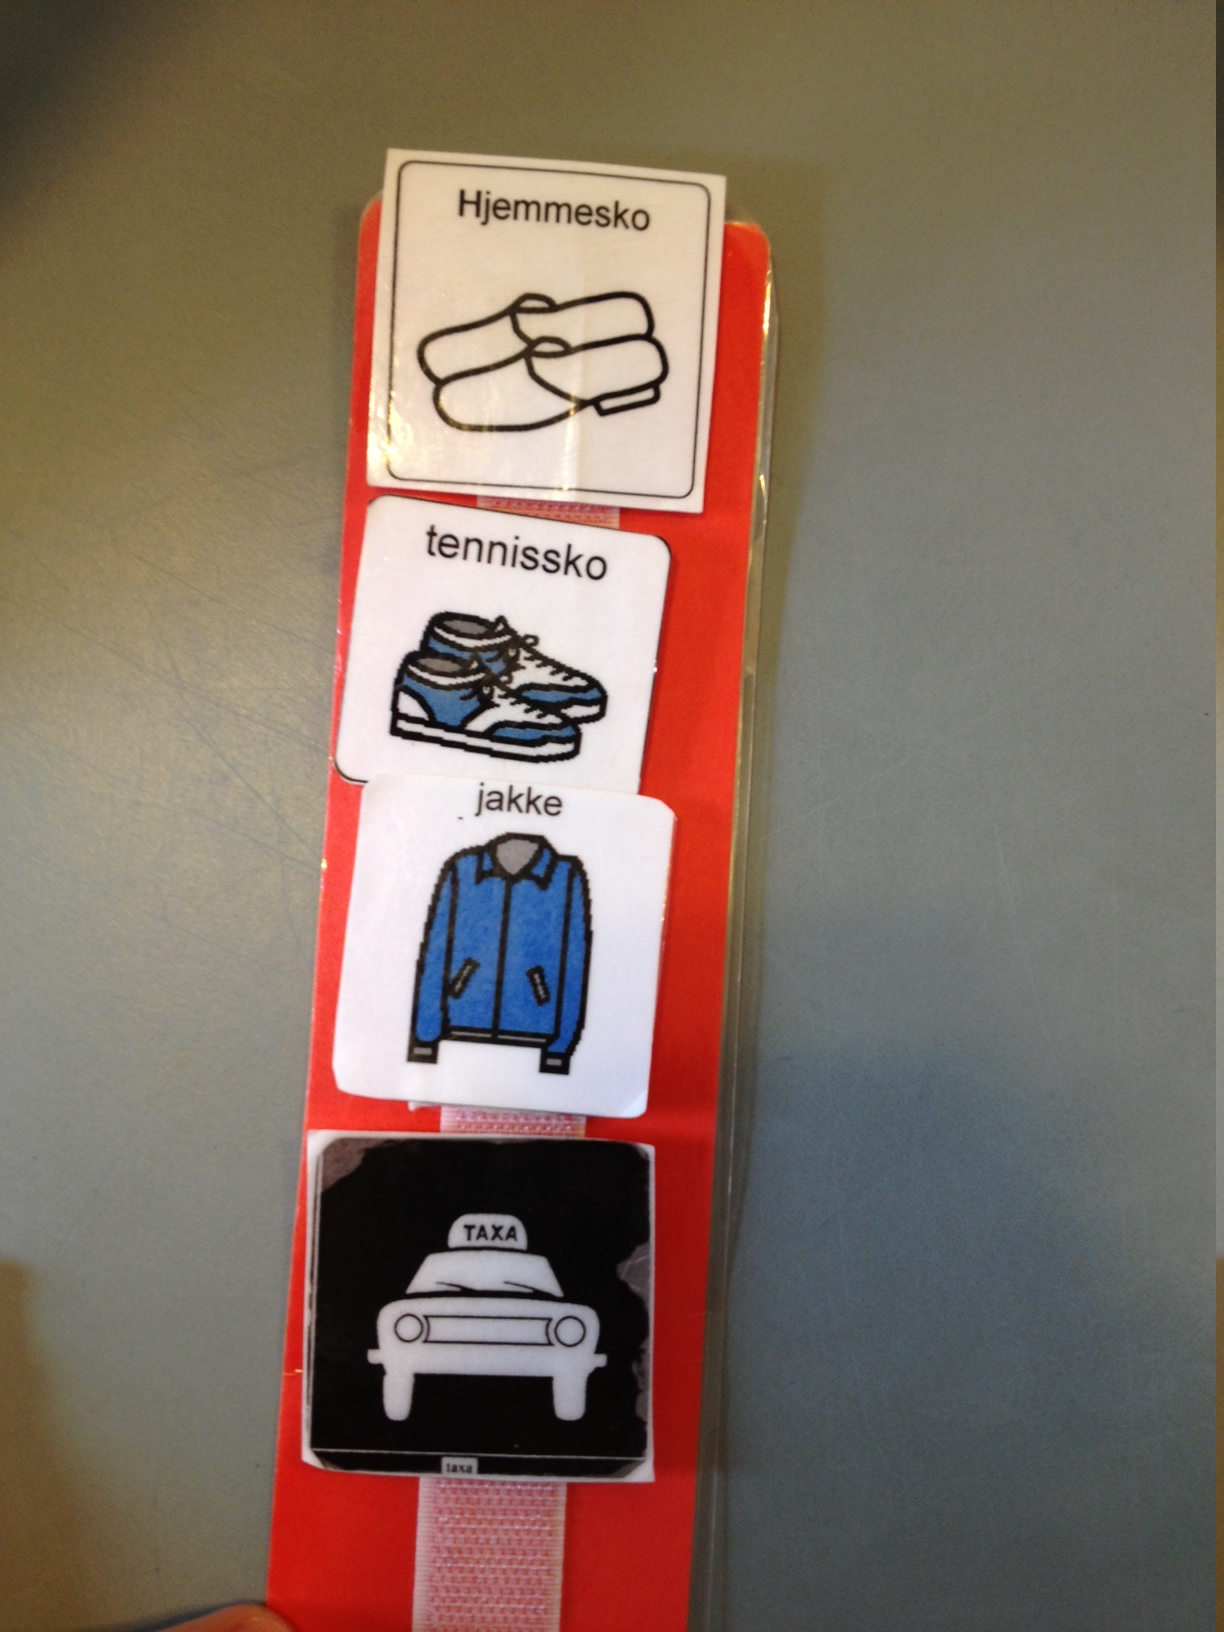
\includegraphics[scale=0.15]{tex/commonReport/img/current_use_picto.jpg}
        \caption{\label{img:pic_current} Pictograms in use 2013}
\end{figure}
During the spring semester of 2013, when this report was written, the use of pictograms is mostly in the form of physical images. The images need to be drawn and/or edited, printed, cut out and then laminated to extend their lifespan. After this process the pictograms are ready for use, generally for one individual, making this repetitive and tedious for the guardians.% \todo{Klim: Bliver dette virkelig kun brugt for et enkelt barn? Kan mapper ikke deles af flere b{\o}rn? Biggi: Nej det kan de ikke, det er blevet sagt af kontakt-person}
When the required amount of pictograms have been created for an individual, they need to be organized and made accessible with the help of some sort of container. This container can be a folder with a pocket for the pictograms and a velcro-like strip for arranging the pictograms. For communication an individual can choose to form sentences by arranging the pictograms accordingly or use a single image to simply express needs and wants. Another purpose of the pictograms can be to graphically represent instructions for various tasks, in the form of ``do \textbf{A}, followed by \textbf{B} and lastly do \textbf{C}'' for individuals requiring special assistance.

\subsubsection*{Digitizing the Pictogram}
%What's new, what had previous groups implemented, reflect on why it had to be redone.
The \ac{giraf} project focuses on simplifying and digitizing a medium used by individuals with autism and their guardians. This includes digitizing the pictograms, making them available on devices running Android with added functionality. Added functionality includes the option to make the pictograms play a sound, dynamically change the layout of text-labels and editing images. Digitizing the pictogram also makes it possible to share them easily, carry them between devices and make backups of them. Previously, with the same idea in mind, it was attempted to digitize the pictogram. It was considered unsatisfactory (see section below) and therefore the re-implementation in this semester's project.

\subsubsection*{GIRAF Pictogram Design}
%What is the pictogram (basically). What are the ideas behind the current design.
%How is this design better than the previous? How is it used?
The digitized pictogram consists of an image, text-label and a sound. With all elements included, it can be presented as each of the three, two parts combined or all three in union. This viewable container is designed as an extension of the \emph{Android} view class, making it easy for developers to include and present in their applications. The idea is to have users sharing the same pictograms, with the option to customize their contents without affecting the pictogram itself. The previous \ac{giraf} pictogram design lacked documentation, portability and functionality such as text-labels. Therefore a new design was implemented, which hopefully fits the needs of both future \ac{giraf} developers and \ac{giraf} users.


\subsection{Morgana}
\label{sub:morgana:intro}
The Morgana library project was initially intended to make it possible for all the \ac{giraf} applications to use both the Wasteland database, see \secref{sub:wasteland}, and the local Oasis database seamlessly, however in the time allotted it was not possible to finish this functionality, so the focus was shifted to making it parse and write \ac{json} objects for use in calls to the Wasteland database.

The library implements a Java class for each value object documented in the Wasteland \ac{api}, each class parses a \ac{json} object and turns it into an object which can be used by \ac{giraf} applications, it is also able to create \ac{json} objects from the stored Java object.


\subsection{Design Guidelines}
\label{sub:designGuidelines}
The purpose with the guidelines is to get a consistent look and feel across all of the different applications included in the \ac{giraf} system.
The design guidelines have been discussed among all of the project groups, and they are as follows:

\begin{quote}
\begin{itemize}
\item Keep the existing color palette
\item Font: Helvetica
\item Font size: use common sense. \emph{Android} offers extra small/small/medium/large/huge
\item Minimize the use of text, use images instead of text
\item \ac{gui} in vector graphics
\item Green and red are universal colors for `accept'/`cancel'
\item Applications have animal icons
\item Icons are non-customizable
\item Every application should be locked in landscape mode
\end{itemize}
\end{quote}

The color palette will be the same as in the 2012 version of \ac{giraf}. With regards to font type and size, Helvetica has been chosen and developers need to keep in mind, that the text has to be readable on the tablet.

The aim is to use more images and less text as the target audience are mostly children, many of which have communication and/or reading difficulties and some have problems imagining objects purely from text.

The \ac{gui} will be in vector graphics, because it scales well, which makes it possible to reuse some of the images. Green and red are universal colors for `accept'/`cancel'. It may sound obvious but other applications have been developed with different colors.
Tool-applications should have animal icons.

Lastly everything will be in landscape mode as this eliminates additional implementation for responsive layout, when the tablet is rotated.


\section{The Project of 2013}
\label{sec:projects}
\subsection{Admin}
\label{sec:admin}
This project focuses on the creation of an administration interface for the \ac{giraf} system. The Admin system consists of two parts, one for a desktop computer and one for \emph{Android}. The desktop part will run on a \ac{lamp} stack and communicate with the database using the database \ac{api} provided by the Wasteland (see \secref{sub:wasteland}) project. The \emph{Android} part will run on the tablet using the same code base as the desktop part, using a web server application. The main focus of the project is for department managers and guardians to be able to administrate the \ac{giraf} system.

\subsection{Cars}
\label{sub:cars}
The aim of the Cars project is to develop an application, which will help children with infantile autism to be more comfortable in using their voice. To ensure that the children learn to use their voice in creating different types of sounds, and not just speak in a monotone way, the application will require the children to create sounds covering different sides of the frequency spectrum.

Cars is a game in which the player has to lead a car through a street into a garage, controlling it with high or low frequency sounds. The car has a matching colored garage at the end, which when entered completes the game successfully.
%The car and garages are colored and the two need to match to successfully complete the game. 
Randomly placed obstacles are used to force the player to avoid them to reach the end.

\subsection{Croc}
\label{sub:Croc}

The Croc project aims to create an application for creation of pictograms for use in the \ac{giraf} system.

\begin{description}
\item  Pictograms can be created in a number of ways:
  \begin{description}
  \item[Camera] take a picture with the camera and turn that picture into a pictogram.
  \item[Drawing] draw a pictogram.
  \item[Audio] record sounds to attach to pictograms.
  \end{description}
\end{description}

\subsection{Parrot}
Parrot is an enhancement of the Parrot project of 2012 and is an application for communication between guardian and child. Its development is based around the currently used physical system \secref{subsub:pic_currentuse}. The original Parrot application from 2012 also included the administration of categories. It was therefore technically possible for a child using Parrot to access these administration tools, and it is for this reason, that the currently developed version has relocated the administration to a separate application named \acl{cat}. The version developed during this project will focus on making improvements to the \ac{gui} design, adding subcategories (such as breakfast item under the food category) and handle the interaction with pictograms. %in such a way, that a long-click is no longer necessary to drag a pictogram to the sentence board.
The primary focus for Parrot remains the same; providing an easier way for children to communicate with guardian in a way that they are familiar with.

\subsubsection*{\acl{cat}}
\label{subsub:cat}
\ac{cat} focuses on administrating categories and subcategories. Currently \ac{cat} is also responsible for communicating with other applications that need specific pictograms, such as the Tortoise (\secref{sub:tortoise}) and Zebra (\secref{sub:zebra}) applications, by providing search/deliver functionality. %Furthermore \ac{cat} handles adding new pictures into categories and subcategories. 
%The primary focus for \ac{cat} is the search/deliver functionality and the administration of categories.

\subsection{Tortoise}
\label{sub:tortoise}
The Tortoise application focuses on helping children learn about their own lives and strengthen their social skills. The hope is, that by letting the child interact with pictures and sentences, that are associated with their life, the child can develop an identity. By developing their own identity, the child will learn how to interact with other people by learning what kind of topics to talk about in a conversation with others.
\subsection{Train}
\label{sub:train}
%Train is a game application for children with autism that is included as a part of the \ac{giraf} project.
The inspiration for Train comes from an exercise, that one of the guardians practices with the children. The purpose of the game is to create a dialogue between the child and the guardian. The child has to drag pictograms from a train station onto the train wagons and make the train drive. When the train arrives at the next station, the child has to drag the correct pictograms from the train and onto the station. The correct pictograms are decided by the station category.

The category for each station is chosen by the guardians by clicking the category picture frame and browsing \ac{cat} (\secref{subsub:cat}) for the picture they want to use. After selecting a category, they select which pictures they want associated with the station. %these are the pictograms the children will have to drag onto the specific station.

\subsection{Wasteland}
\label{sub:wasteland}
The purpose of the Wasteland project is to handle all of the data for the \ac{giraf} system. In order to achieve this goal, a database will be implemented on a central server and a local database will be kept on the tablet. The two databases will synchronize data on a regular basis.
\subsection{Zebra}
\label{sub:zebra}
The aim of the Zebra project is to create a software application aiding guardians in their work. The application should aid the guardian in situations where a child is to perform an ordered sequence of actions. These actions are typically represented by pictograms. %that the child understands\todo{kan der ikke findes et bedre ord?}.
Zebra should replace the current paper based version of this system. The guardian should be able to create and manage digital versions of such sequences specific to each child. Upon selecting a sequence for the child to follow, the child should be able to mark actions as done when they are completed to illustrate their progress.

%% \subsection{Morgana}
\label{sub:morgana:intro}
The Morgana library project was initially intended to make it possible for all the \ac{giraf} applications to use both the Wasteland database, see \secref{sub:wasteland}, and the local Oasis database seamlessly, however in the time allotted it was not possible to finish this functionality, so the focus was shifted to making it parse and write \ac{json} objects for use in calls to the Wasteland database.

The library implements a Java class for each value object documented in the Wasteland \ac{api}, each class parses a \ac{json} object and turns it into an object which can be used by \ac{giraf} applications, it is also able to create \ac{json} objects from the stored Java object.


%%
% List of projects
%

% \section{Future work}

%%
% List of future work
%

\section{Acknowledgement}
The group of students working with \ac{giraf} during the spring semester of 2013, would like to thank the contacts, who were;

\begin{description}
\item [Tove S{\o}by] - speech therapist, and contact for three groups.
\item [Mette Als Andreasen] - kindergarten teacher at Birken Langholt, and contact for two groups.
\item [Kristine Niss Henriksen] - kindergarten teacher at Birken Vodskov, and contact for one group.
\item [Drazenko Banjak] - teacher at Egebakken Vodskov, and contact for one group.
\item [Mette Frost] - teacher at Egebakken Vodskov, and contact for one group.
\end{description}

In addition the group would like to thank Ulrik Nyman, semester coordinator, for his help, guidance and engagement during the project.

	
\chapter{User Manual}

\emph{(Chapter introduction goes here)}
\chapter{User Manual}

\emph{(Chapter introduction goes here)}
\chapter{User Manual}

\emph{(Chapter introduction goes here)}
\chapter{User Manual}

\emph{(Chapter introduction goes here)}
\chapter{User Manual}

\emph{(Chapter introduction goes here)}
\chapter{User Manual}

\emph{(Chapter introduction goes here)}
\chapter{User Manual}

\emph{(Chapter introduction goes here)}
\chapter{User Manual}

\emph{(Chapter introduction goes here)}

\bookmarksetup{startatroot}% dette skulle stoppe part, så conclusion får indryk. Problemet i skrivende øjeblik er at chapters har samme indryk uafhængigt af parts
\addtocontents{toc}{\bigskip}%laver ekstra mellemrum

\cleardoublepage
\begin{appendices}
\chapter{API Documentation}\label{app:api}
  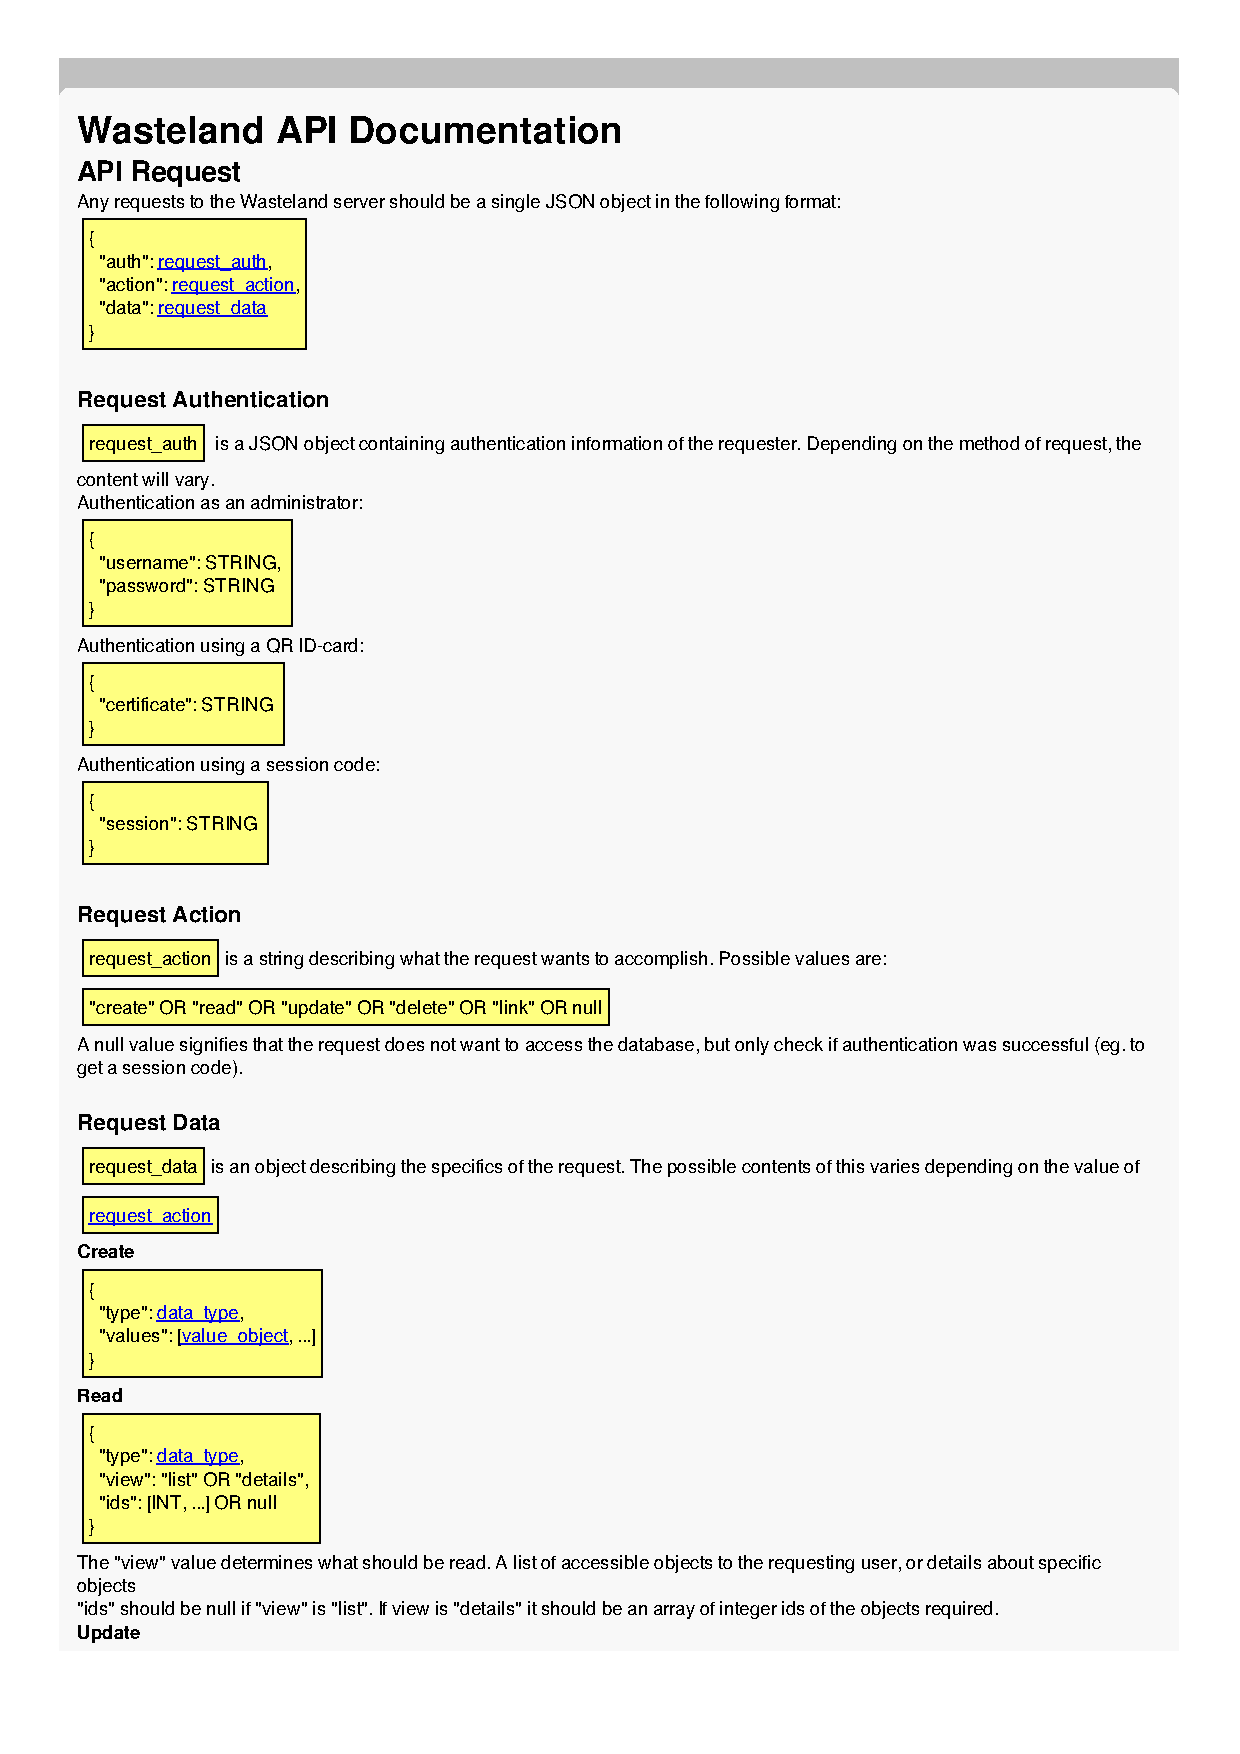
\includepdf[pages={1}]{img/appendix_api}
  \includepdf[pages={2}]{img/appendix_api}
  \includepdf[pages={3}]{img/appendix_api}
  \includepdf[pages={4}]{img/appendix_api}
  \includepdf[pages={5}]{img/appendix_api}
\chapter{Unit Test Example}\label{app:unit_test}
  \lstinputlisting[language=c++]{lst/unit_test_example.cpp}
\end{appendices}
\cleardoublepage
\pdfbookmark{Bibliography}{bib}
\bibliographystyle{plain}
\bibliography{bib/bibliography,tex/commonReport/bib/commonReport}

\end{document}
